\documentclass[10pt,reqno]{amsart}
\usepackage[left=1in,right=1in,top=1in,bottom=1.25in]{geometry}%

\usepackage{setspace}
\usepackage[utf8]{inputenc}
\usepackage[usenames,dvipsnames]{xcolor}
\usepackage{mdwlist}
\usepackage{caption}
\usepackage{subcaption}

% AMS packages
\usepackage{amsmath}
\usepackage{amssymb}
\usepackage{amsthm}
\usepackage{mathtools}
\usepackage{graphicx}
\usepackage{enumerate}
\usepackage{float}
\usepackage{subfiles}

% my custom packages
\usepackage{macros}
\usepackage{packages}
\usepackage{style}

\theoremstyle{plain}
\newtheorem{theorem}{Theorem}
\newtheorem{corollary}[theorem]{Corollary}
\newtheorem{lemma}[theorem]{Lemma}

\theoremstyle{definition}
\newtheorem{definition}[theorem]{Definition}
\newtheorem{example}[theorem]{Example}

\theoremstyle{remark}
\newtheorem{remark}[theorem]{Remark}
\newtheorem{hypothesis}[theorem]{Hypothesis} 

\numberwithin{theorem}{section}
\numberwithin{equation}{section}

\begin{document}

\section{Krein bubble}

\subsection{Block matrix for periodic 2-pulse}

Using the symmetry of the periodic 2-pulse, the block matrix $S(\lambda)$ and the determinant $E(\lambda) = \det S(\lambda)$ has the following form.

\begin{lemma}\label{lemma:2blockmatrix}
For a periodic 2-pulse, the block matrix $S(\lambda)$ is the $4 \times 4$ matrix
\begin{align}\label{dpSmatrix}
S(\lambda) = 
\begin{pmatrix}
e^{-\nu(\lambda)X_1} & -e^{\nu(\lambda)X_0} & \tilde{M}^c \lambda^2 & 0 \\
-e^{\nu(\lambda)X_1} & e^{-\nu(\lambda)X_0} & 0 & \tilde{M}^c \lambda^2 \\
\frac{1}{2}\lambda M^c e^{-\nu(\lambda)X_1} & \frac{1}{2}\lambda M^ce^{\nu(\lambda)X_0} &-a-\lambda^2 M & a \\
\frac{1}{2}\lambda M^c e^{\nu(\lambda)X_1} & \frac{1}{2}\lambda M^c e^{-\nu(\lambda)X_0}  & a & -a-\lambda^2 M
\end{pmatrix} + R(\lambda)
\end{align}
where
\begin{equation}\label{2pa}
a = \langle \Psi(X_0), Q'(-X_0) \rangle + \langle \Psi(X_1), Q'(-X_1) \rangle.
\end{equation}
The remainder matrix is a $4 \times 4$ matrix of the form
\begin{align}
R(\lambda)
\begin{pmatrix} 
c_1(\lambda) & \tilde{c}_1(\lambda) & \lambda d_1(\lambda) & \lambda \tilde{d}_1(\lambda) \\ 
-c_1(-\lambda) & -\tilde{c}_1(-\lambda) & -\lambda \tilde{d}_1(-\lambda) & -\lambda d_1(-\lambda) \\ 
c_2(\lambda) & \tilde{c}_2(\lambda) & d_2(\lambda) & \tilde{d}_2(\lambda) \\ 
-c_2(-\lambda) & -\tilde{c}_2(-\lambda) & \tilde{d}_2(-\lambda) & d_2(-\lambda)
\end{pmatrix},
\end{align}
where the individual entries have bounds
\begin{align*}
|c_1|, |\tilde{c}_1| &\leq C (|\lambda| + r^{1/2})^2, \quad |d_1|, |\tilde{d}_1| \leq C (|\lambda| + r^{1/2})^2 \\
|c_2|, |\tilde{c}_2| &\leq C (|\lambda| + r^{1/2})^2, \quad |d_2|, |\tilde{d}_2| \leq C (|\lambda| + r^{1/2})^3
\end{align*}
In addition,
\begin{equation}\label{2pblockmatrixdet}
\begin{aligned}
\det S(&\lambda, r) = -2 \lambda^2 (2a + \lambda^2 M + R_1) \left( M \sinh(\nu(\lambda)X) + \lambda (M \tilde{M} - M^c \tilde{M}^c) \cosh(\nu(\lambda)X) \right) \\
&-4 a \lambda^3 M^c \tilde{M}^c \sinh(\nu(\lambda)X_1)\sinh(\nu(\lambda)X_0) 
+ R_2 \lambda^2 \sinh(\nu(\lambda)(X_1 - X_0)) + \lambda^2 R_3 \sinh(\nu(\lambda)X)) + \lambda^3 R_4,
\end{aligned}
\end{equation}
where the $R_i$ are scalars with bounds 
\begin{equation*}
|R_1| \leq C r^{3/2}, \quad |R_2|, |R_3|, |R_4| \leq C(|\lambda| + r^{1/2})^4,
\end{equation*}
and $\det S(-\lambda) = -\det S(\lambda)$.
\end{lemma}

The Krein bubble occurs when first essential spectrum eigenvalue (positive Krein signature) collides with imaginary interaction eigenvalue (negative Krein signature) on the imaginary axis. These are, to leading order, given by
\begin{align*}
\lambda_1 &= c \frac{\pi i}{X + c \frac{M\tilde{M} - M^c\tilde{M^c}}{M}} \\
\lambda_* &= \sqrt{-\frac{2a}{M}}.
\end{align*}
Recall that $X = X_0 + X_1$, and we can change $X$ by changing $X_1$ without changing the scaling factor $r$. $X_0$ and $X_1$ are related, but for sufficiently large $X_1$, varying $X_1$ produces essentially no change in $X_0$. Thus since $\lambda_* = \mathcal{O}(e^{-\alpha X_0}) = \mathcal{O}(r^{1/2})$, $\lambda_*$ is essentially constant for what we will be doing. Also we assume $\lambda_*$ is purely imaginary, since that is the interesting case.

We will need something a little better for $\lambda_*$. Since the remainder term $R_1 = \mathcal{O}(r^{3/2})$ and (importantly) does not depend on $\lambda$, take instead
\begin{equation}\label{lambdastar}
\lambda_* = \sqrt{-\frac{2a - R_1 }{M}} = \sqrt{-\frac{2a}{M}} + \mathcal{O}(r).
\end{equation}
which will eliminate a term we don't want later.

Change variables by letting $\mu = \nu(\lambda)$. For sufficiently small $\lambda$, we then have
\begin{equation}\label{lambdamu}
\lambda = \nu^{-1}(\mu) = c \mu + \mathcal{O}(\mu^3),
\end{equation}
which gives us the expression
\begin{equation}\label{det2}
\begin{aligned}
\det S(&\mu, r) = -2 c^2 \mu^2 (2a + c^2 \mu^2 M + R_1) \left( M \sinh(\mu X) + c \mu K \cosh(\mu X) \right) \\
&-4 a c^3 \mu^3 M^c \tilde{M}^c \sinh(\mu X_1)\sinh(\mu X_0) 
+ R_2 \mu^2 \sinh(\mu(X_1 - X_0)) + \mu^2 R_3 \sinh(\mu X) + \mu^3 R_4,
\end{aligned}
\end{equation}
where $K = M \tilde{M} - M^c \tilde{M}^c$. Since we are looking for nonzero eigenvalues, we can divide by $c^2 \mu^2$ to solve
\begin{equation}\label{det3}
\begin{aligned}
-2 (&2a + c^2 \mu^2 M + R_1) \left( M \sinh(\mu X) + c \mu K \cosh(\mu X) \right) \\
&-4 a c \mu M^c \tilde{M}^c \sinh(\mu X_1)\sinh(\mu X_0) 
+ R_2 \sinh(\mu(X_1 - X_0)) + R_3 \sinh(\mu X) + \mu R_4 = 0
\end{aligned}
\end{equation}
where $K = M \tilde{M} - M^c \tilde{M}^c$.

\subsection{Leading order terms}

Since the Krein bubble is centered around the imaginary essential spectrum eigenvalue, let $\mu_* = \lambda_* / c$ and $\mu_1 = \lambda_1 /c$. For our ansatz, we take
\[
\mu = \mu_* + h
\]
The maximum radius of the Krein bubble happens when $\lambda_1 = \lambda_*$. We can always choose $X$ so that this occurs. Define the parameter $k$ by
\[
\mu_1 = \mu_* - k i,
\]
so that 
\[
\mu = \mu_1 + k i + h.
\]
The parameter $k$ measures the distance between $\mu_1$ and $\mu_*$ on the imaginary axis. The maximum radius will occur when $k = 0$. 

We now substitute our ansatz into \cref{det2}. First, we have
\[
2a + c^2 \left(\mu_* + h \right)^2 M + R_1 = 2 c^2 M \mu_* h  + M c^2 h^2.
\]
We note that our choice of $\lambda_*$ eliminates $R_1$ here, which is key. Expanding the denominator of $\mu_1$ in a Taylor series,
\begin{align*}
\mu_1 &= \frac{\pi i}{X\left(1  + c \frac{K}{M X} \right) }
= \frac{\pi i}{X}\left( 1 - c \frac{K}{M X} + c^2 \frac{K^2}{M^2 X^2} + \mathcal{O}\left(\frac{1}{X^3}\right) \right).
\end{align*}
Substituting $\mu = \mu_1 + k i + h$ and expanding the $\sinh$ and $\cosh$ terms in a Taylor series about $\pi i$,
\begin{align*}
\sinh(\mu X) &= \sinh\left( \pi i - c \frac{K \pi i }{M X} + c^2 \frac{K^2 \pi i }{M^2 X^2} + (h + k i)X + \mathcal{O}\left(\frac{1}{X^3}\right) \right) \\
&= (-1)\left( - c \frac{K \pi i }{MX} + c^2 \frac{K^2 \pi i }{M^2 X^2} + (h + k i)X \right) + \mathcal{O}\left( \left(\frac{1}{X} + (h + k) X \right)^3 \right)
\end{align*}
and
\begin{align*}
\cosh(\mu X) &= \cosh\left( \pi i - c \frac{K \pi i }{M X} + c^2 \frac{K^2 \pi i }{M^2 X^2} + (h + k i)X + \mathcal{O}\left(\frac{1}{X^3}\right) \right) \\
&= (-1) + \mathcal{O}\left( \left(\frac{1}{X} + (h + k)X \right)^2 \right)
\end{align*}
Thus we have
\begin{align*}
M \sinh(&\mu X) + c \mu K \cosh(\mu X) \\
&= -M \left( -c \frac{K \pi i }{MX} + c^2 \frac{K^2 \pi i }{M^2 X^2} + (h + k i)X \right) + \mathcal{O}\left( \left(\frac{1}{X} + (h + k)X \right)^3 \right) \\
&- K \left( \frac{c \pi i}{X} - c^2 \frac{K \pi i}{M X^2} + c^3 \frac{K^2 \pi i}{M^2 X^3} + c (h + k i) + \mathcal{O}\left(\frac{1}{X^3}\right) \right)\left( -1 + \mathcal{O}\left( \left(\frac{1}{X} + (h + k)X \right)^2 \right) \right) \\
&= -\left( M + \frac{c K}{X}\right)(h+ki)X + \mathcal{O}\left( \left( \frac{1}{X} + (h+k)X \right)^3 \right)
\end{align*}

\subsection{Rescaling}

Anticipating what we will get in the end, we take the following rescaling.
\begin{align*}
\mu_* &= r^{1/2} \tilde{\mu} \\
h &= r^{5/4} X_0 \tilde{h}  \\
k &= r^{5/4} \tilde{k} 
\end{align*}
Since $\mu_1$ is close to $\mu_*$, $1/X = \mathcal{O}(r^{1/2})$, thus $\sinh(\mu X) =  \mathcal{O}(r^{1/2})$. Furthermore, 
\begin{align*}
\sinh(\mu&(X_1 - X_0)) = \sinh(\mu(X - 2 X_0)) \\
&= \sinh(\mu X) \cosh(2 \mu X_0)  - \cosh(\mu X)\sinh(2 \mu X_0) \\
&= \mathcal{O}\left( r^{1/2} + r^{1/2} X_0 \right) 
= \mathcal{O}\left( r^{1/2}|\log r| \right) 
\end{align*}
Finally, 
\begin{align*}
\sinh(\mu &X_1)\sinh(\mu X_0) = \sinh(\mu ( X - X_0 )) \sinh(\nu(\lambda)X_0) \\
&= \left( \sinh(\mu X) \cosh( \mu X_0)  - \cosh(\mu X)\sinh(\mu X_0) \right)\sinh(\mu X_0) \\
&= \mu_*^2 X_0^2 + \mathcal{O}(r^{1/2})
\end{align*}

Substituting these into \cref{det3} and simplifying, we wish to solve
\begin{equation}\label{det4}
\begin{aligned}
2 &\left( 2 c^2 M \tilde{\mu} \tilde{h} X_0 r^{7/4} \right) 
\left( \left( M + \frac{c K}{X} \right) X ( \tilde{h} + \tilde{k} i) X_0 r^{5/4} + \mathcal{O}(r^{3/2}) \right) 
+ 2 M M^c \tilde{M}^c c^3 \tilde{\mu}^5 r^{5/2} X_0^2 + \mathcal{O}( r^{5/2} |\log r| ) = 0
\end{aligned}
\end{equation}
Since
\[
\left( M + \frac{c K}{X} \right) X  = MX + c K = \frac{M \pi}{\lambda_1} = \frac{M \pi}{c \mu_*}
= \frac{M \pi}{c \tilde{\mu}r^{1/2}}
\]
at the center of the Krein bubble, this simplifies to
\begin{equation}\label{det4}
\begin{aligned}
4 \pi c M^2 X_0 r^{7/4} \tilde{h} \left( ( \tilde{h} + \tilde{k} i) X_0 r^{3/4} + \mathcal{O}(r) \right) 
+ 2 M M^c \tilde{M}^c c^3 \tilde{\mu}^5 r^{5/2} X_0^2 + \mathcal{O}( r^{5/2} |\log r| ) = 0
\end{aligned}
\end{equation}

Dividing by $X_0^2 r^{5/2}$ and noting that $X_0 = \mathcal{O}(|\log r|)$, we obtain the equation
\begin{equation}\label{det5}
\begin{aligned}
\tilde{h} ( \tilde{h}+ \tilde{k} i) 
+ \frac{M^c \tilde{M}^c }{2 \pi M^2 } c^2 \tilde{\mu}^5 + \mathcal{O}\left( \frac{1}{|\log r|} \right) = 0,
\end{aligned}
\end{equation}
where we used the fact that $1/|\log r|$ is lower order than $r^{1/2}$. We can use this to prove the Krein bubble exists and persists for small $r$. To do this, we use the IFT to show that happens everywhere except for where the eigenvalues collide on the imaginary axis. For the collision point, we use the IFT again to show that there is a double zero of this function, which must then be on the imaginary axis by Hamiltonian symmetry.

Undoing the scaling and changing variables back to $\lambda$, the Krein bubble is centered at $\lambda_*$ and has radius (in the complex plane) of $\lambda = \sqrt{R}$, where 
\begin{equation}\label{Kreinrad}
R = -\frac{M^c \tilde{M}^c }{2 \pi c M^2 } \lambda_*^5 X_0^2.
\end{equation}
Since $M^c$ and $\tilde{M}^c$ have opposite signs, $R > 0$, so the radius is real. (In fact, numerics suggest that $\tilde{M}^c = -M^c$, although I have no idea if we can show that. Probably not.) 

\subsection{Numerics}

We cannot (unfortunately) do nice decay estimates for this on KdV5, since we can only construct the first periodic 2-pulse with imaginary eigenvalues to a sufficient degree of accuracy for AUTO. The issue is that the tails of the primary pulse decay too fast, and the tail oscillations of the primary pulse are too slow, so that the tail interactions become negligible too quickly.

To get around this problem, we instead look at this ``contrived'' version of KdV5.
\begin{equation}\label{KdV5alt}
u_t = \partial_x\left( u_{xxxx} - 2(a-b)u_{xx} + (a+b)^2 u - u^2 \right),
\end{equation}
which is constructed so that eigenvalues of the background state are 0 and $\pm \sqrt{a} \pm \sqrt{b}$. Thus we can manipulate $a$ and $b$ to control the background eigenvalues. In particular, this lets us construct the first 4 periodic 2-pulses with imaginary interaction eigenvalues so we can find the Krein bubble using AUTO and then get decay estimates on the size of the Krein bubble. A plot of the relative error of the Krein bubble radius (using the formula above) vs. $\alpha X_0$ is shown in \cref{fig:Kreinrelerror}, which suggests that the remainder term is order $e^{-3 \alpha X_0}$, which is higher order than the Krein bubble radius! The relative error for the fourth periodic double pulse is less than 0.01.

\begin{figure}
\begin{center}
\begin{tabular}{c}
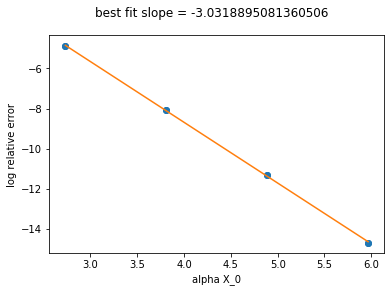
\includegraphics[width=7.5cm]{images/Kreinrelerror.png}
\end{tabular}
\end{center}
\caption{Log relative error of Krein bubble radius vs. $\alpha X_0$ for first four double pulse solutions to \cref{KdV5alt} with imaginary interaction eigenvalues. $a = 0.35$, $b = 3$. }
\label{fig:Kreinrelerror}
\end{figure}


\end{document}